
\documentclass[../D+Manual.tex]{subfiles}
\begin{document}

\chapter{Symmetries} \label{chp:Symmetries}

\begin{quote}
	
	
	The universe is built on a plan the profound symmetry of which is somehow present in the inner structure of our intellect.\\
	\hspace*{\fill} \textit{Paul Valery}
\end{quote}

\section{Introduction}

Supramolecular complex structures can be often described as hierarchical data trees in which repeating subunits are docked into their assembly symmetries. The assembly symmetries describe how repeating subunits are organized (in other words, translated and rotated) is space (see Figure \ref{fig:hierarchical}). For complex assemblies, the scattering amplitude is given by: 

\begin{equation}
\label{eqn:assemblyScatteringAmplitude}
F\left(\vec{q}\right)=
\sum_{j=1}^{J}
\sum_{m=1}^{M_j}
\left[F_{j}\left(\mathbf{A}_{j,m}^{-1}\vec{q}\right)\cdot
\exp\left(i\vec{q}\cdot\vec{R}_{j,m}\right)\right]
\end{equation}
where $F\left(\vec{q}\right)$ is the scattering amplitude from an assembly comprised of $n_s$ subunits. $J$ is the number of different types of objects, which is also the total number of leaves in the hierarchical tree structure representation of the entire supramolecular assembly (Figure \ref{fig:hierarchical}). The leaves can either be geometry-based or atomic-based models, taken, for example, from Protein Data Bank (PDB) files. 
$M_j$ is the number of instances of object type $j$, whose orientations and positions are determined by rotation matrices  $\mathbf{A}_{j,m}$ (see section \ref{sec:symmetryEditor}) and real-space translation vectors $\vec{R}_{j,m}$, respectively. The total number of subunits, $n_s$, is therefore  $\sum_{j=1}^{J}{M_j}$.

To evaluate the scattering of a complex structure, we need a way to describe ``Assembly Symmetries''. In D+, there are three methods to do so.



\begin{figure}[h]
	\centering
%	\tikzsetnextfilename{Tree}	% name next TikZ figure
	\usetikzlibrary{shapes,snakes}

\begin{tikzpicture}[
every node/.style={inner sep=2pt},
level/.style={sibling distance=65mm/#1},
root/.append style={ellipse,draw,fill=blue!30},
symm/.append style={ellipse,draw,fill=yellow!30},
 pdb/.append style={ellipse,draw,fill=black!10},
 ]
\node [root](rt){Supramolecular Assembly}
	child{node[symm](s1){$\text{Assembly}_1$}
		child{node[pdb](p1){$\text{Subunit}_1$}}
		child{node[symm](s2){$\text{Assembly}_2$}
			child{node[pdb](p2){$\text{Subunit}_2$}}
		}
	}
	child{node[symm](s3){$\text{Assembly}_3$}
		child{node[pdb](p3){$\text{Subunit}_3$}}
		child{node[pdb](p4){$\text{Subunit}_4$}}
	}
;
\path (s1) -- (s3) node [scale=3,midway] {$\hdots$};
\path (p3) -- (p4) node [scale=1.5,midway] {$\hdots$};
\path (p1) -- (s2) node [scale=1.5,midway] {$\hdots$};
\end{tikzpicture}
	% input TiKZ figure code - See more at: http://www.howtotex.com/tips-tricks/faster-latex-part-ii-external-tikz-library/#sthash.daLZMQjk.dpuf
%	\includegraphics[width=\linewidth]{Tree}
	\caption {Example of modeling a supramolecular assembly in a hierarchical manner. Each \textit{Assembly Symmetry}  may contain multiple children. Children can either be additional \textit{Assembly Symmetries} or \textit{Subunits}. A \textit{Subunit} represents an atomic model (for example, a Protein Data Bank (PDB) file) or a geometric model. Internal nodes consist of \textit{Assembly Symmetries}, whereas each leaf must be a \textit{Subunit}.  There may be an arbitrary number of hierarchy levels and nodes in each level. Many supramolecular structures may be constructed that way. Care, however, should be taken when dealing with very large structures (see \hyperref[sec:hybrid]{\textbf{Hybrid Calculations}} for details).}
	\label{fig:hierarchical}
\end{figure}


\section{Space-Filling Symmetry}
\subsection{Background}
\begin{figure} %[6]{r}{0.5\textwidth}
	\centering
	\tikzsetnextfilename{BasisVector}	% name next TikZ figure
	\usetikzlibrary{shapes,snakes}

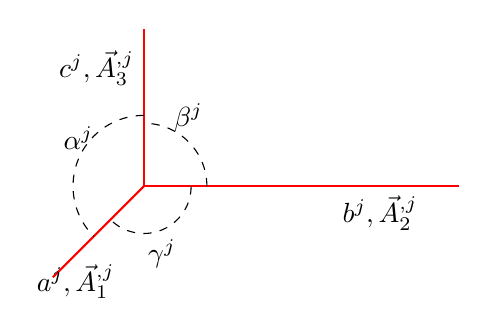
\begin{tikzpicture}
\coordinate (O) at (0,0,0);
\coordinate (A) at (4,0,0);
\coordinate (B) at (0,2,0);
\coordinate (C) at (0,0,3);
\draw[thick,red] (O) -- (A);
\draw[thick,red] (O) -- (B);
\draw[thick,red] (O) -- (C);
\path (O)+(0,0,0) -- (A)+(0,0,0) node [near end, below] {$b^j,  \vec{A}^{,j}_2$};
\path (O)+(0,0,0) -- (B)+(0,0,0) node [near end, left] {$c^j,  \vec{A}^{,j}_3$};
\path (O)+(0,0,0) -- (C)+(0,0,0) node [near end, below] {$a^j,  \vec{A}^{,j}_1$};
\draw[dashed,-](0.6,0,0) arc(0:-135:0.6) node[midway,below]{$\gamma^j$};
\draw[dashed,-](0.8,0,0) arc(0:90:0.8) node[midway,above]{$\beta^j$};
\draw[dashed,-](0,0.9,0) arc(90:225:0.9) node[midway,above]{$\alpha^j$};
%\draw[thick,-] (A) arc - (B);
%\draw[dashed] (\rvec,0,0) arc (0:90:\rvec);
%\draw[thick,->] (0,0,0) --  (2,0,0) node[anchor=north east]{$a$}(aVec);
%\draw[thick,->] (0,0,0) -- (0,2,0) node[anchor=north west]{$b$}(bVec);
%\draw[thick,->] (0,0,0) -- (0,0,2) node[anchor=south]{$c$}(cVec);
\end{tikzpicture}
	% input TiKZ figure code - See more at: http://www.howtotex.com/tips-tricks/faster-latex-part-ii-external-tikz-library/#sthash.daLZMQjk.dpuf
	\caption{Unit cell vectors. $a^j$ is the length of $\vec{A}^{,j}_1$, which is laying along the $x$-axis, $b^j$ is the length of $\vec{A}^{,j}_2$, which is within the $xy$ plane, and $c^j$ is the length of $\vec{A}^{,j}_3$. The angles between the unit cell vectors are indicated in the Figure.}
	\label{fig:unitcellvectors}
\end{figure}

In this method, all child subunits are treated as a unit cell of a primitive Bravais lattice. Copies of unit cell object type $j$ at the same orientation, given by  matrix $\mathbf{A}_{j}$, are placed at $R_{j,m}=R^j_{n^j_1,n^j_2,n^j_3}=n^j_1\cdot\vec{A}^j_1+n^j_2\cdot\vec{A}^j_2+n^j_3\cdot\vec{A}^j_3$, where $m$ is an index that  corresponds to $\left\lbrace n^j_1,n^j_2,n^j_3\right\rbrace$, which is any combination of three integers between $\left\lbrace 0,0,0\right\rbrace$ and  $\left\lbrace\left( N_1^{j}-1\right),\left(N_2^{j}-1\right),\left(N_3^{j}-1\right)\right\rbrace$.
The unit cell vectors, $\vec{A}^j_1,\vec{A}^j_2$, and $\vec{A}^j_3$ are defined by three lengths $a^j,b^j$, and $c^j$ and three angles $\alpha^j,\beta^j$, and $\gamma^j$ (Figure \ref{fig:unitcellvectors}).
The total number of subunit copies, $M_j$, of object $j$ will be $N_1^{j}\times N_2^{j}\times N_3^{j}$. The contribution of the space-filling lattice, comprise of repeating subunits of type $j$, to the scattering amplitude, $F_J$, is computed according to:
\begin{equation}
\label{eqn:assemblyScatteringAmplitudeSFS}
F_J\left(\vec{q}\right)=
F_{j}\left(\mathbf{A}_{j}^{-1}\vec{q}\right)\cdot\exp\left(i\vec{q}\cdot\vec{T}_{j}\right)\cdot SF^j(\vec{q}),
\end{equation}
where $\mathbf{A}_{j}$ is the rotation matrix by which subunit $j$ was rotated, $\vec{T}_j$ is a translation vector of the  entire space-filling lattice, and $SF^j(\vec{q})$ is the space-filling structure-factor, given by:
\begin{equation}
\label{eqn:assemblyScatteringSFS}
SF^j(\vec{q})=
\overset{\left(N_{1}^{j}-1\right)}{\underset{n^{j}_{1}=0}{\sum}}\overset{\left(N_{2}^{j}-1\right)}{\underset{n^{j}_{2}=0}{\sum}}\overset{\left(N_{3}^{j}-1\right)}{\underset{n^{j}_{3}=0}{\sum}}\exp\left(i\vec{q}\cdot\vec{R}^j_{n^{j}_{1},n^{j}_{2},n^{j}_{3}}\right).
\end{equation} 

The three unit vectors in real-space are constructed in the following way. We start with vector $\vec{A}^{j}_{1}$ of
length $a^j$ along the $x$ direction and vector $\vec{A}^{j}_{2}$ of length
$b^j$. The angle between the two vectors is $\gamma^j$. We then
add a third vector $\vec{A}^{j}_{3}$ defined by its length $c^j$
and two more angles $\alpha^j$ and $\beta^j$, where $\alpha^j$ is between
the vectors $\vec{A}^{j}_{1}$ and $\vec{A}^{j}_{3}$, and $\beta^j$ is between
the vectors $\vec{A}^{j}_{2}$ and $\vec{A}^{j}_{3}$. In real-space, the basis
vectors are given by:

\begin{equation*}
\vec{A}^{j}_{1}=(a^j,0,0),
\end{equation*}


\begin{equation*}
\vec{A}^{j}_{2}=\left(b^j\cos\gamma^j,b^j\sin\gamma^j,0\right),
\end{equation*}


\begin{equation*}
\vec{A}^{j}_{3}=\left(c^j\cos\alpha^j,\frac{c^j\cdot t^j}{\sin\gamma^j},\frac{c^j\cdot B^j}{\sin\gamma^j}\right),
\end{equation*}
where $t^j=\cos\beta^j-\cos\alpha^j\cos\gamma^j$ and  $B^j=\sqrt{\sin^{2}\gamma^j-\sin^{2}\gamma^j\cos^{2}\alpha^j-\left(t^j\right)^{2}}$. 

The angles should satisfy the conditions that the sum of any pair of angles is larger (or equal) than the third angle and that $\sin\gamma^j \neq 0$ and $\sin^{2}\gamma^j-\sin^{2}\gamma^j\cos^{2}\alpha^j-\left(t^j\right)^{2} > 0$.  D+ checks that these conditions are satisfied. If the sum of two angles equals the third angle, or if $\sin\gamma^j = 0$, the symmetry is 2D.
In this case, the correct usage of the D+ is to project the 2D symmetry on the \plane{x}{y}. The projection is done by providing the values of $a^j$, $b^j$, and $\gamma^j$, set both $\alpha^j$ and $\beta^j$ to be 90, and set the number of repeating subunits in the third $(z)$ direction to be 1.

In real-space, the unit cell vectors $\vec{A}_{h}$ can then be rotated by a rotation matrix $\mathbf{O}_j$, so that the final unit cell vectors are: $\vec{a}_{h}^j=\mathbf{O}_j\vec{A}_{h}^{j}$, where $h\in\left\{ 1,2,3\right\}$, and then $R_{j,m}=R^j_{n^j_1,n^j_2,n^j_3}=n^j_1\cdot\vec{a}^j_1+n^j_2\cdot\vec{a}^j_2+n^j_3\cdot\vec{a}^j_3$. 



\subsubsection{What can we expect to find in reciprocal-space?}

 As the basis vectors in reciprocal space are given by:
\begin{equation*}
\vec{a}_{1}^{*j}=\frac{2\pi}{\upsilon ^j}\cdot\left(\vec{a}^j_2\times\vec{a}^j_3\right),\,  \vec{a}_{2}^{*j}=\frac{2\pi}{\upsilon ^j}\cdot\left(\vec{a}^j_3\times\vec{a}^j_1\right),\, \vec{a}_{3}^{*j}=\frac{2\pi}{\upsilon ^j}\cdot\left(\vec{a}^j_1\times\vec{a}^j_2\right) 
\end{equation*}
where $\upsilon ^j=\vec{a}^j_1\cdot\left(\vec{a}^j_2\times\vec{a}^j_3\right)$, we get:


\begin{equation*}
\vec{a}_{1}^{*j}=\left(\frac{2\pi}{a^j},\frac{-2\pi\cos\gamma^j}{a^j\sin\gamma^j},\frac{2\pi\left(t^j\cdot\cos\gamma^j-\cos\alpha^j\sin^{2}\gamma^j\right)}{a^j\cdot B^j\sin\gamma^j}\right),
\end{equation*}


\begin{equation*}
\vec{a}_{2}^{*j}=\left(0,\frac{2\pi}{b\sin\gamma^j},\frac{-2\pi t^j}{b^j\cdot B^j\sin\gamma^j}\right),
\end{equation*}


\begin{equation*}
\vec{a}_{3}^{*j}=\left(0,0,\frac{2\pi\sin\gamma^j}{c^j\cdot B^j}\right).
\end{equation*}

Any $\vec{q}$-vector, which is a linear combination of the reciprocal-space basis-vector, and is given by
\begin{equation*}
\vec{G}^j_{h_j,k_j,l_j}=h_j\vec{a}_{1}^{*j}+k_j\vec{a}_{2}^{*j}+l_j\vec{a}_{3}^{*j},
\end{equation*}
where $h_j,k_j$, and $l_j$ are integers, satisfies Bragg's condition, hence contributes (according to equation \ref{eqn:assemblyScatteringSFS}) to a structure-factor correlation peak at $\vec{q}=\vec{G}^j_{h_j,k_j,l_j}$. In solution, the contribution of $SF^j$ to the scattering curve will be at the scattering-vector amplitudes, $q$, which satisfy Bragg's condition, and are given by:

\begin{equation*}
q=\left|\vec{G}^j_{h_j,k_j,l_j}\right|=\left|h_j\vec{a}_{1}^{*j}+k_j\vec{a}_{2}^{*j}+l_j\vec{a}_{3}^{*j}\right|=
\end{equation*}
\begin{equation*}
\frac{2\pi}{a^j\cdot b^j\sin\gamma^j}\cdot
\sqrt{\begin{array}{c}
\left(h_jb^j\sin\gamma^j\right)^{2}+\left(k^j\cdot a^j-h_j\cdot b^j\cos\gamma^j\right)^{2}+\\
\frac{\left(h_jb^jc^j\left(\cos\gamma^j\cos\beta^j-\cos\alpha^j\right)-k_ja^jc^j\left(\cos\beta^j-\cos\alpha^j\cos\gamma^j\right)+l_ja^jb^j\sin^{2}\gamma^j\right)^{2}}{\left(c^j\right)^{2}\left(\sin^{2}\gamma^j-\cos^{2}\alpha^j-\cos^{2}\beta^j+2\cos\beta^j\cos\alpha^j\cos\gamma^j\right)}
\end{array}}.
\end{equation*}

\noindent The line-shape of the peaks will follow Equations \ref{eqn:assemblyScatteringAmplitudeSFS} and \ref{eq:OE}.

Space-filling is a relatively easy way to create a regular Bravais lattice. For example, a 3D hexagonal lattice is defined by:

\begin{equation*}
\left\lbrace a^j = b^j ,c^j, \alpha^j = \beta^j = 90\degree, \gamma^j = 120\degree \right\rbrace
\end{equation*}

\noindent Figure \ref*{fig:3Dhexagonal} shows an example of a 3D hexagonal lattice with five repeats in each direction.

\begin{figure} %[6]{r}{0.4\textwidth}

	%\vspace{-10pt}
	\centering
	%\fbox{
	%l b r t
    \includegraphics[trim={115pt 180pt 15pt 230pt},clip,width=0.45\linewidth]{"Hexagonal Lattice"}
    %}
	%\vspace{-20pt}
	\caption{Example of a 3D hexagonal lattice.}
	\label{fig:3Dhexagonal}
\end{figure}

\subsection{Using Space-Filling Symmetry in D+}
To use space-filling symmetry in D+, go to \path{Domain View}, select \path{Space-filling Symmetry}, and press \path{Add}. Then select the subunit model to which the space-filling symmetry applies and drug it with the mouse into the relevant \path{Space-filling symmetry}. To edit the parameters of the space-filling symmetry, select it and edit the values in the \path{Parameter Editor} of the space-filling symmetry, which looks as shown here. The input parameters include the three lattice distances $a^j, b^j$, and $c^j$, the three lattice angles (in degrees) $\alpha^j, \beta^j$, and $\gamma^j$, as well as the number of subunit \path{Repetitions} in each of the three lattice \path{Vector}s.  

\begin{wrapfigure}{r}{0.6\textwidth}
	\vspace{-15pt}
	\centering
    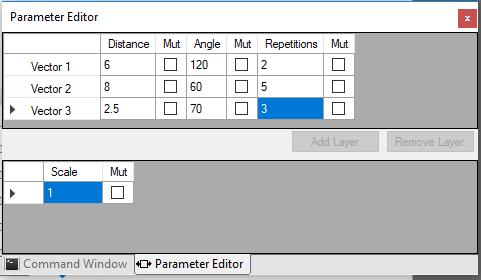
\includegraphics[width=0.95\linewidth]{SpaceFillingSymmetry}
\end{wrapfigure}
\begin{wrapfigure}{r}{0.6\textwidth}
	\vspace{-15pt}
	\centering
    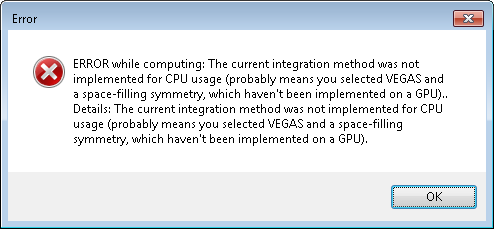
\includegraphics[width=0.95\linewidth]{Error_VEGAS_with_Space_Filling_Not_Hybrid_GPU.png}
\end{wrapfigure}

\texttt{Space Filing Symmetry} does not automatically center the structure around the origin. To facilitate easer calculations, it is suggested to wrap the entire structure in a \texttt{Manual symmetry}, and place the center of mass of the entire structure approximately at the origin.
Note: An error message will appear when trying to use \texttt{Grids} for \texttt{Space Filling Symmetry} (which was implemented only for CPU) of a PDB file, and compute orientation average using VEGAS Monte Carlo (implemented only for GPU). This computation, however, can be done using the Hybrid or Direct methods. If geometric models are used (instead of a PDB), the computation can be done.






  
\section{Manual Symmetry}
\label{sec:ManualSymmetry}

\begin{wrapfigure}{r}{0.6\textwidth}
	\vspace{-15pt}
	\centering
    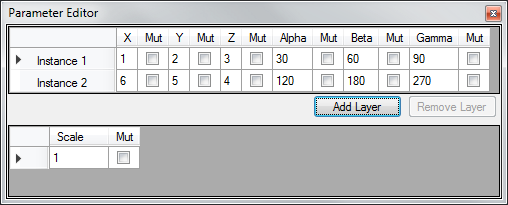
\includegraphics[width=0.95\linewidth]{ParameterEditorManualSymmetry}
\end{wrapfigure}



Any three dimensional object in 3D space can be positioned and rotated by a set of six parameters: $\left\lbrace x,y,z\right\rbrace$ to determine its displacement and $\left\lbrace\alpha, \beta, \gamma\right\rbrace$ as Euler angles for rotation. A \texttt{Manual Symmetry} is a table of these six parameters per object. In the \texttt{Parameter Editor} Figure shown, there are two copies of children (\texttt{Instance 1} and \texttt{Instance 2}) at two arbitrary positions and orientations. The list of coordinates and orientations can be loaded from a ``Docking List'' (DOL) text file (\texttt{*.dol}) only after adding a \texttt{Manual Symmetry}. The file should be tab or space delimited with each row starting with an index, followed by $\left\lbrace x,y,z\right\rbrace$ and finishing with $\left\lbrace \alpha, \beta, \gamma\right\rbrace$. A file that would create the \texttt{Manual Symmetry} in the image would look like:

\begin{lstlisting}[basicstyle=\small,breaklines=false,backgroundcolor=\color{gray!15}]
1	1	2	3	30	60	90
2	6	5	4	120	180	270
\end{lstlisting}

Note: The indices at the beginning of each line have no meaning, they just need to be integers.

\section{Scripted Symmetry}
\label{sec:ScriptedSymmetry}
%TODO add more examples and explanations. 

\lstset{style=Luastyle,}

A scripted symmetry is a \href{http://www.lua.org/}{\texttt{Lua}} script that creates a \hyperref [sec:ManualSymmetry] {Manual Symmetry} behind the scenes based on parameters provided by the user.
The \href{http://www.lua.org/}{\texttt{Lua}} script has to contain an \lstinline|Information| Table and several functions that will be presented below.
We shall run through an example script to show the usage.

\subsection{\lstinline|Information| Table}
\begin{sloppypar}
The \lstinline|Information| Table has five fields: \lstinline|Name|; \lstinline|Type|; number of layer parameters \lstinline|(NLP)| ; \lstinline|MinLayers|; \lstinline|MaxLayers|. 
\end{sloppypar}

\begin{lstlisting}[basicstyle = \small]
Information = {
    Name = "Simple Grid in XY",  -- This is the name that will be displayed in the Domain View
    Type = "Symmetry", -- This is the type, should be "Symmetry" for scripted symmetries
    NLP = 2, -- Number of Layer Parameters: The number of parameters per layer
    MinLayers = 2, -- The minimal number of layers (<= MaxLayers)
    MaxLayers = 2, -- The maximal number of layers (>= MinLayers)
};
\end{lstlisting}

The parameters provided by the user are organized in layers, in each layer the same number of parameters \lstinline|(NLP)|. (defining  \lstinline|MaxLayers| to be $-1$ enables the user to control the number of layers from the GUI)

\subsection{\lstinline|Populate| Function}
Next, several functions need to be added. The first function to implement is the workhouse of the script. It populates the \hyperref [sec:ManualSymmetry] {\texttt{Manual Symmetry}}.
\begin{lstlisting}[basicstyle = \small,literate={'}{{'}}1,escapeinside={(*}{*)}]
function Populate(p, nlayers)
    -- This is really just a sanity check, but doesn't hurt to add it.	
	if (p == nil or nlayers (*$\sim$*)= 2 or table.getn(p[1]) (*$\sim$*)= 2) then				
		error("Parameter matrix must be 7x1, it is " .. nlayers .. "x" .. table.getn(p[1]));
	end
	
\end{lstlisting}
This is a check for the correct size of the parameter matrix, the number of layers (nlayers) and the number of parameters in each layer (table.getn(p[1]))

\begin{lstlisting}[basicstyle = \small,literate={'}{{'}}1,escapeinside={(*}{*)}]
	-- Create meaningful names
	DistanceX    = p[1][1];
	DistanceY    = p[2][1];
	RepetitionsX = p[1][2];
	RepetitionsY = p[2][2];
	

	-- Create the table to return, and the indices
	res = {};
	n = 1;


	-- Fill the res table to papulate Manual Symmetry
	
	for y = 1, RepetitionsY	 do
			for x = 1, RepetitionsX	 do
				res[n] = {DistanceX*(x-RepetitionsX/2-0.5),
			   			 DistanceY*(y-RepetitionsY/2-0.5),
						  0,0,0,0};
						  
					n = n + 1;
			end
	end
	
	-- Return the complete table of x,y,z, \alpha, \beta, \gamma
	return res;

end
\end{lstlisting}

\noindent notice that to reduce the \texttt{Grid Size} required for accurate calculations, we were careful to center the complete object around the origin.

\subsection{\lstinline|GetLayerName| Function}
There are a few additional functions that are required for the user interface (UI). It needs to know things about variables like \texttt{Layer} and \texttt{Parameter Names}, is it applicable, and default values. For starters, the text displayed to the left of the table in Figure \ref{fig:ParameterEditor} (section \ref{sec:parameterEditor}) is generated with the function below. Each row (or layer) gets the text based on its index, as shown.

\begin{lstlisting}[basicstyle = \small]
function GetLayerName(index)
	if index == 0 then
		return "X";
	elseif index == 1 then
		return "Y";
	
	else	
		return "N/A";
	end
end

\end{lstlisting}

\subsection{\lstinline|GetLayerParameterName| Function}
Next, the text above the table in Figure \ref{fig:ParameterEditor} is obtained with the function below. Each column (or layer parameter) gets the text based on its index, as shown.
\begin{lstlisting}[basicstyle = \small]
function GetLayerParameterName(index)
	if index == 0 then
		return "distance";
		elseif index == 1 then
		return "Repetitions";
	else
		return "N/A"
	end
end
\end{lstlisting}

\subsection{\lstinline|IsParamApplicable| Function}
The applicability of a parameter is less obvious in this example. Here, all the parameters are applicable, so the function is a straightforward \lstinline|return true;|.

\begin{lstlisting}[basicstyle = \small]
function IsParamApplicable(layer, layerParam)
	return true;
end
\end{lstlisting}

\begin{wrapfigure}{r}{0.3\textwidth}
	\vspace{-10pt}
	\centering
    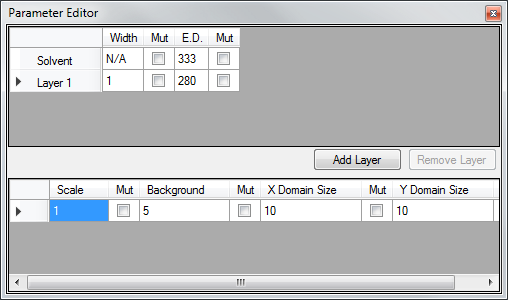
\includegraphics[trim={7pt 210pt 269pt 25pt},clip,width=0.95\linewidth]{ParameterEditorSlabs}
\end{wrapfigure}

A better (theoretical) example would be as shown in the image here. In this example, the \texttt{Solvent} layer does not have a \texttt{Width}. So the function should return true for all options \textit{except} when both \lstinline|layer| and \lstinline|layerParam| equal zero.

\begin{lstlisting}[basicstyle = \small]
function IsParamApplicable(layer, layerParam)
	if (layer == 0 and layerParam == 0) then
		return false;
	return true;
end
\end{lstlisting}

\subsection{\lstinline|GetDefaultValue| Function}
Finally, the UI needs to have some default values for each of the \lstinline|layer| -  \lstinline|layerParam| combinations.

\begin{lstlisting}[basicstyle = \small]
function GetDefaultValue(layer, layerParam)
	if layer == 0 then
		if layerParam == 0 then
			return 1;
		elseif layerParam == 1 then
			return 10;
		end
	elseif layer == 1 then
		if layerParam == 0 then
			return 1;
		elseif layerParam == 1 then
			return 10;
		end
	
	end
end
\end{lstlisting}



\end{document}


